% V2 figures; paths are relative to this analysis directory.
\begin{figure}[t]\centering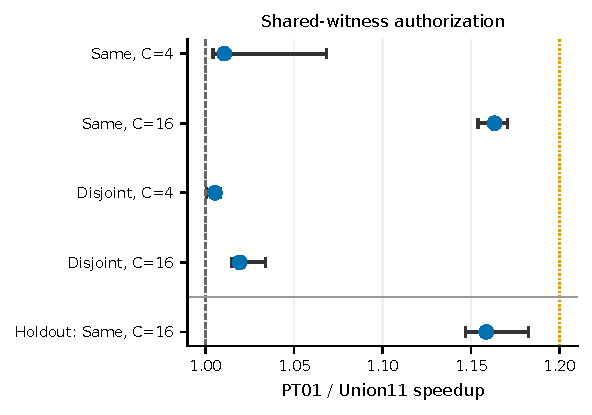
\includegraphics[width=\columnwidth]{figures/fig1_primary_speedup.pdf}\caption{PT01-to-Union11 authorization speedup with 95\% seed-cluster bootstrap intervals.}\label{fig:v2-speedup}\end{figure}
\begin{figure}[t]\centering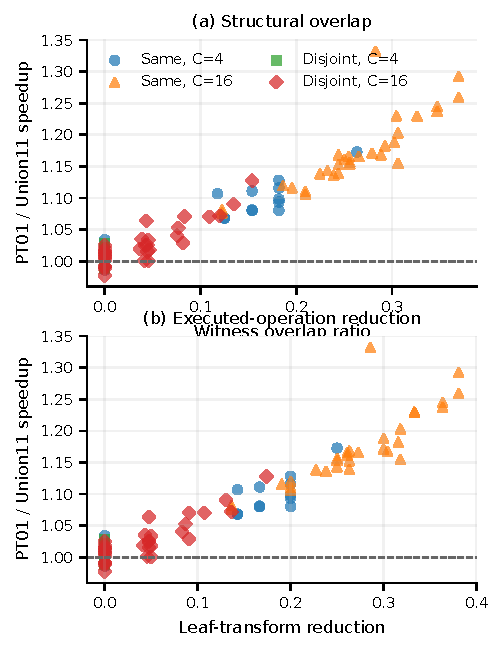
\includegraphics[width=\columnwidth]{figures/fig2_overlap_reuse.pdf}\caption{Instance-level witness overlap, executed-operation reduction, and paired speedup.}\label{fig:v2-overlap}\end{figure}
\begin{figure}[t]\centering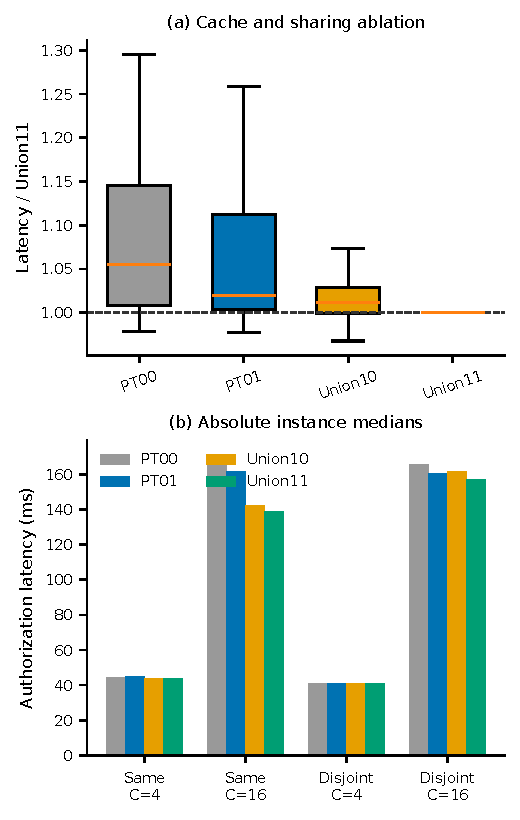
\includegraphics[width=\columnwidth]{figures/fig3_ablation.pdf}\caption{Header-cache and shared-witness ablation.}\label{fig:v2-ablation}\end{figure}
\begin{figure}[t]\centering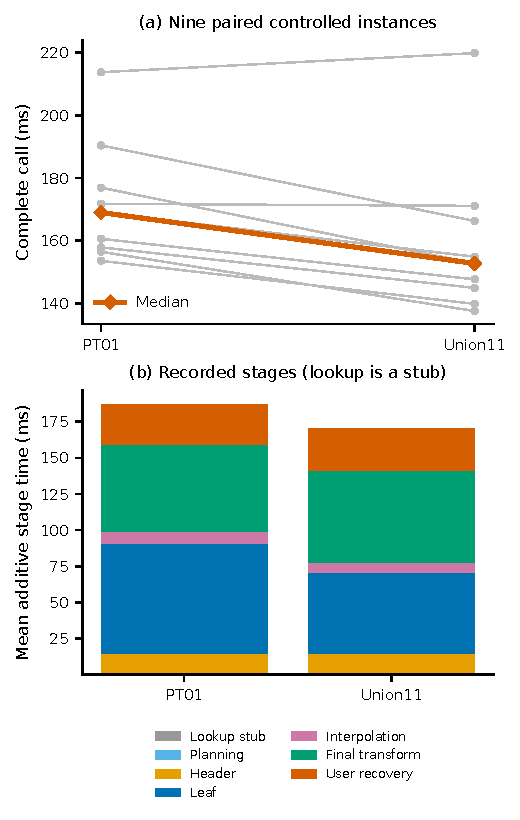
\includegraphics[width=\columnwidth]{figures/fig4_end_to_end.pdf}\caption{Controlled complete-call latency and recorded stage means.}\label{fig:v2-e2e}\end{figure}
\begin{figure}[t]\centering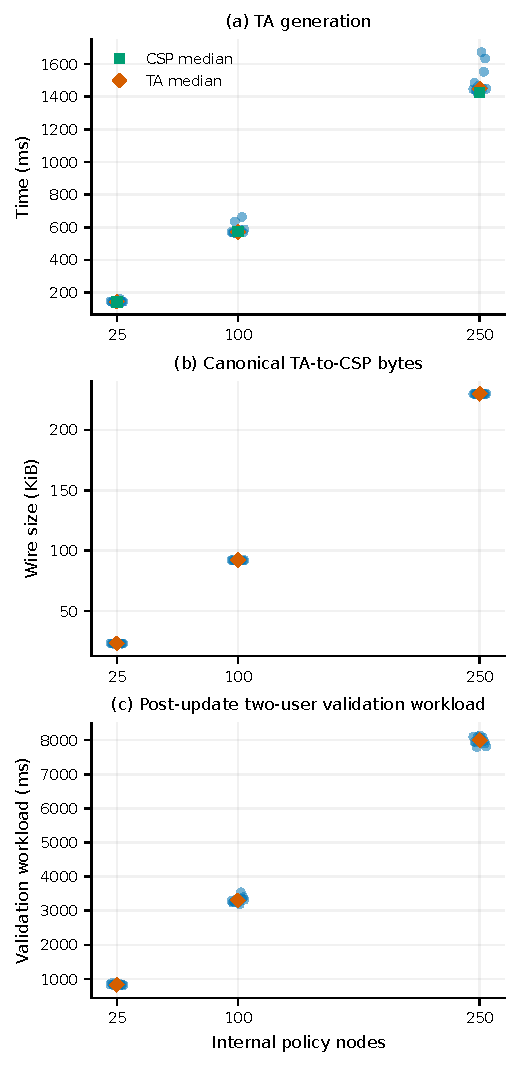
\includegraphics[width=\columnwidth]{figures/fig5_revocation.pdf}\caption{Attribute-revocation update costs and canonical transfer size.}\label{fig:v2-revocation}\end{figure}
\begin{figure}[t]\centering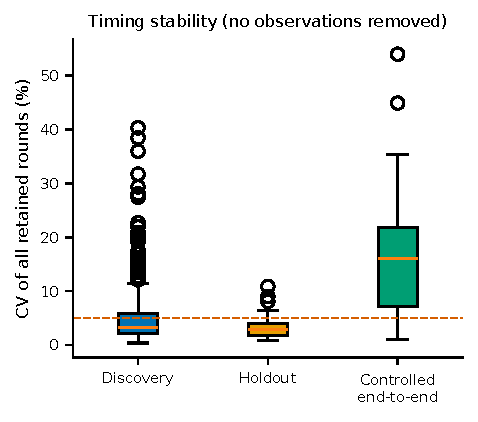
\includegraphics[width=\columnwidth]{figures/fig6_timing_stability.pdf}\caption{CV across all retained timing rounds.}\label{fig:v2-stability}\end{figure}
